\documentclass[14pt]{extarticle}
\usepackage[utf8]{inputenc}
\usepackage[spanish]{babel}
\usepackage{enumerate}
\usepackage{graphicx}
\usepackage[hidelinks]{hyperref}
\usepackage[vmargin=2cm,hmargin=2cm]{geometry}

\begin{document}

\thispagestyle{empty}

\noindent\rule[-1ex]{\textwidth}{2pt}\\[4.5ex]

D.\textbf{Alejandro J. León Salas}, Profesor del Departamento de Lenguajes y Sistemas Informáticos de la Universidad de Granada.\\

D.\textbf{Antonio Martínez López}, Profesor del Departamento de Geometría y Topología de la Universidad de Granada.\\

\vspace{0.5cm}

\textbf{Informan:}

\vspace{0.5cm}

Que el presente trabajo, titulado \textit{\textbf{Entendiendo la teoría de nudos mediante la simulación y la informática gráfica}},
ha sido realizado bajo su supervisión por \textbf{Cristina Zuheros Montes}, y autoriza la defensa de dicho trabajo ante el tribunal
que corresponda.

\vspace{0.5cm}

Y para que conste, expide y firma el presente informe en Granada a 13 de diciembre de 2016.

\vspace{1cm}

\textbf{Los directores:}

\vspace{1cm}

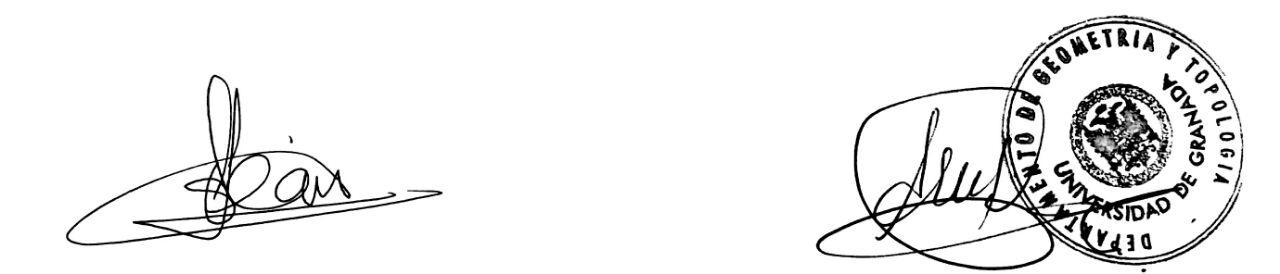
\includegraphics[width=1\textwidth]{firmaTutores.jpg}\\
\noindent \textbf{Alejandro J. León Salas} \hspace{6cm} \textbf{Antonio Martínez López}
\end{document}
